%Bliver lavet overgang i Purpose. 
\section{Zinc homeostatis and efflux pumps in \textit{P. aeruginosa}}

Trace elements, such as zinc, are necessary for normal cell function, due to the fact that they are used as cofactors in many proteins \cite{Blencowe2003ZnIIProkaryotes}\cite{McCall2000FunctionMetalloenzymes}. Zinc is further used to regulate smaller molecules and potentially DNA as well \cite{Nejdl2014DNAIons} (and as reviewed by \cite{Krezel2016TheIons}). As a result, zinc is necessary for many of \textit{P. aeruginosa}’s virulence factors such as biofilm formation and swarming motility \cite{Mastropasqua2018EfficientLung}.

\subsection{\textit{P. aeruginosa} under zinc starvation}

Since zinc is necessary for both cellular and bacterial growth, the spread of pathogens can be reduced through decreasing levels of zinc (and other nutrients). This process is called nutritional immunity, and is imposed by the human immune system. Nutritional immunity, in relation to zinc, is achieved through zinc-chelation by proteins such as the metallophore calprotectin (as reviewed by \cite{Gonzalez2019PseudomonasPathogen}). This is the case in the lungs of cystic fibrosis patients infected by \textit{P. aeruginosa}. Here  high levels of calprotectin is a contributor to low levels of free zinc ions \cite{Gray2012SputumDiseases}. However \textit{P. aeruginosa} can still thrive and express zinc dependent virulence factors \cite{Mastropasqua2018EfficientLung}. \textit{P. aeruginosa} achieves this through at least three different systems, which help the pathogen maintain zinc homeostasis. These systems are as follows: 

\begin{itemize}
    \item \textit{P. aeruginosa} has a few different transport systems for the uptake of free zinc ions. One of these systems consists of three outer membrane pumps which can import zinc to the periplasmic space (PA0781, P11922, PA4837) \cite{Pederick2015ZnuAAeruginosa}. The transport of zinc in its free form, from the periplasmic space into the cytoplasm, is achieved through the known ZnuABC system and possibly the PA4063-PA4066 system \cite{Pederick2015ZnuAAeruginosa}\cite{Fiorillo2021StructureAeruginosa}. These different pumps helps increase the concentration of zinc in the cytoplasm, in relation to the outer environment.
    
    \item There is evidence for \textit{P. aeruginosa} being able to produce a metallophore which binds zinc. The chelated zinc-metallophore complex can then be transported into \textit{P. aeruginosa}. Hence \textit{P. aeruginosa} can compete with the host over the free zinc ions \cite{Mastropasqua2017GrowthMetallophore}.
    
    \item \textit{P. areugionsa} can produce paralogous proteins, that can replace other zinc dependent proteins. This will in turn increase available zinc (as reviewed by \cite{Gonzalez2019PseudomonasPathogen}). As an example, \textit{P. aeruginosa} can produce two paralogous proteins replacing two “zinc dependent” 50S ribosomal proteins. This releases a high amount of bound zinc in the bacteria, thereby increasing the concentration of available zinc \cite{Lim2013ThePf-5}.
\end{itemize}

\subsection{\textit{P. aeruginosa} under high zinc concentrations}
The former mentioned systems makes it possible for \textit{P. areugionsa} to survive zinc depleted conditions. Furthermore \textit{P. areugionsa} has the ability to survive high levels of zinc. This ability helps the bacterium with undermining the immune system as high zinc concentrations is used as a defense mechanism \cite{Botella2011MycobacterialMacrophages}. The high concentration of zinc is toxic as it causes mismetaliations in proteins. This results in inhibition of set proteins which have great effect on different essential pathways. It is know that zinc is used as signal during infection but whether not the zinc intoxication is an evolved mechanism is yet to be known \cite{McDevitt2011AZinc}. 

\textit{P. areugionsa} can survive high zinc concentrations through systems of efflux pumps. In  \textit{P. areugionsa} the efflux pump removing zinc from the cell interior is the CzcCBA pump. The CzcCBA efflux pump is a RND type efflux pump. The RND type efflux pumps consist of a proton antiporter located in the cytoplasmic membrane, a membrane fusion protein located through the periplasmic space, and an outer membrane protein \cite{Perron2004CzcR-CzcSAeruginosa}. This makes it possible to move the zinc from interior to the outside of the bacteria. 
The presence of zinc induces both the transcription of the \textit{czcCBA} operon and the regulatory genes \textit{czcR} \& \textit{czcS}. This makes it even harder to treat infections with \textit{P. aeruginosa} as they are dependent on the zinc concentration. 

The regulatory gene \textit{czcR} is responsible for regulating the \textit{oprD} gene \cite{Perron2004CzcR-CzcSAeruginosa}. The \textit{oprD} gene is interesting as it codes for the protein porin generally responsible for the influx of carbapenems (beta-lactam antibiotics) in gram-negative bacteria. The CzcR protein negatively regulate the expression of \textit{oprD} can result in imipenem resistant to carbapenems. It is only the dephosphorylated CzcR that can negatively regulate the expression of \textit{oprD}. The phosphorylated CzcR is necessary for triggering the transcription of the \textit{czcCBA} operon \cite{Perron2004CzcR-CzcSAeruginosa}. Whether the CzcR is phosphorylated or not, depends on the activity of CzcS as it is a histidine kinase. Histidine kinase has involvement in the dimerization, phosphotransfer, and phosphatase activity. In \textit{P. aeruginosa} two mutations were found in CzcS resulting in the protein primarily being autophosporylated. These mutations were placed in the link between the two domains in CzcS thus lowering the phosphate activity. The aforementioned lessens the dephosphorylation of CzcR resulting in a higher transcription rate of the \textit{czcCBA} operon (figure \ref{figureefflux}). The high transcription rate makes it possible to remove the toxic amount of zinc in the bacteria \cite{Perron2004CzcR-CzcSAeruginosa}. 

\begin{figure}[H]
\centering
    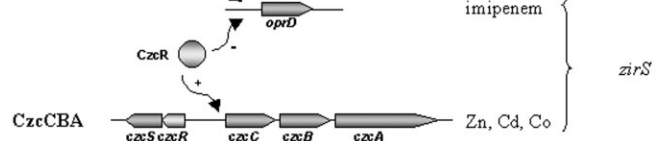
\includegraphics[width=0.80\textwidth]{Figures/Efflux figure.png}
    \caption{\footnotesize{The two operons is seen on the left hand side, where the \textit{oprD} operon is at the top and the \textit{czcCBA} operon at the bottom. When the \textit{oprD} operon is negatively regulated by CzcR the impenem antibiotic resistance is achieved. The possible regulation of the \textit{oprD} operon and the \textit{CzCBA} operon by CzcR protein is shown in middle \cite{Perron2004CzcR-CzcSAeruginosa}.}}
    \label{figureefflux}
\end{figure}

\noindent All of these tools make \textit{P. aeruginosa} able to thrive and express virulence factors under zinc starvation and in excess of zinc. Another virulence factor of \textit{P. aeruginosa} is the zinc dependent biofilm production which will be further discussed in the next section.
